\documentclass[crop,tikz]{standalone}
\usetikzlibrary{backgrounds}
\colorlet{blue}{cyan}
\tikzset{
  inverted/.style = {
    color=white,
    background rectangle/.style={fill},
    show background rectangle
  }
}

\usetikzlibrary{decorations.markings}
\usepackage{pgfplots}
\pgfplotsset{compat=1.17}
\tikzset{>=latex}

\pgfplotsset{
  inverted/.style = {
    every axis legend/.append style={
      draw=white,
      fill=black,
      text=white
    }
  },
  every non boxed x axis/.append style={
    axis line style={-latex}
  },
  every non boxed y axis/.append style={
    axis line style={-latex}
  },
}


\begin{document}
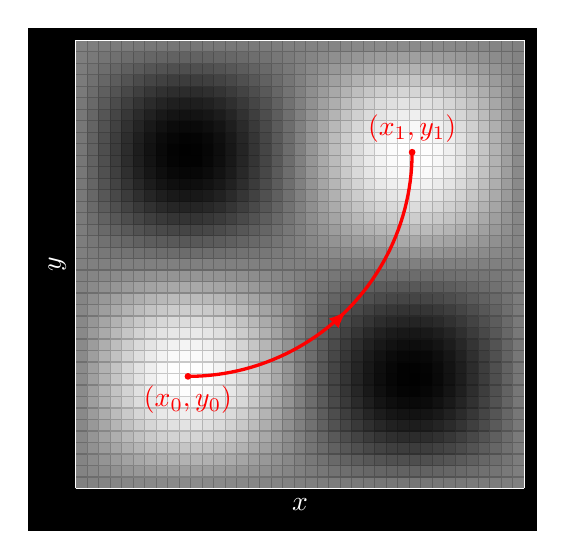
\begin{tikzpicture}[inverted,inverted]
  \pgfmathsetmacro{\px}{pi/2}; % start x coordinate
  \pgfmathsetmacro{\py}{pi/2}; % start y coordinate
  \pgfmathsetmacro{\qx}{3*pi/2}; % end x coordinate
  \pgfmathsetmacro{\qy}{3*pi/2}; % end y coordinate
  \begin{axis}[inverted,
    view={0}{90},
    xlabel={$x$},
    ylabel={$y$},
    axis equal image,
    xtick=\empty,
    ytick=\empty,
    xmin=0,xmax={2*pi},
    ymin=0,ymax={2*pi},
    declare function = {
      f(\x,\y) = sin(deg(x))*sin(deg(y));
    },
    samples=40, samples y=40,
    domain=0:{2*pi}, domain y=0:{2*pi},
    ]
    \addplot3[surf,colormap/blackwhite] { f(x, y) };
    \addplot[red,
      very thick,
      domain={-pi/2}:{0},
      samples=50,
      decoration={markings, mark=at position 0.5 with {\arrow{>}}},
      postaction={decorate}] ({\px+pi*cos(deg(x))},{\qx+pi*sin(deg(x))});
    % marks
    \addplot[only marks, mark=*, mark size=1pt, red] coordinates { ({\px}, {\py}) } node[below] { $(x_0, y_0)$ };
    \addplot[only marks, mark=*, mark size=1pt, red] coordinates { ({\qx}, {\qy}) } node[above] { $(x_1, y_1)$ };
  \end{axis}
\end{tikzpicture}
\end{document}
